\documentclass[ucs,9pt]{beamer}

% Copyright 2004 by Till Tantau <tantau@users.sourceforge.net>.
%
% In principle, this file can be redistributed and/or modified under
% the terms of the GNU Public License, version 2.
%
% However, this file is supposed to be a template to be modified
% for your own needs. For this reason, if you use this file as a
% template and not specifically distribute it as part of a another
% package/program, I grant the extra permission to freely copy and
% modify this file as you see fit and even to delete this copyright
% notice.
%
% Modified by Tobias G. Pfeiffer <tobias.pfeiffer@math.fu-berlin.de>
% to show usage of some features specific to the FU Berlin template.

% remove this line and the "ucs" option to the documentclass when your editor is not utf8-capable
\usepackage[utf8x]{inputenc}    % to make utf-8 input possible
\usepackage[english]{babel}     % hyphenation etc., alternatively use 'german' as parameter
\usepackage{graphicx}
\usepackage{subcaption}
\captionsetup{compatibility=false}


% Template for talks using the Corporate Design of the Freie Universitaet
%   Berlin, created following the guidelines on www.fu-berlin.de/cd by
%   Tobias G. Pfeiffer, <tobias.pfeiffer@math.fu-berlin.de>
% This file can be redistributed and/or modified in any way you like.
%   If you feel you have done significant improvements to this template,
%   please consider providing your modified version to
%   https://www.mi.fu-berlin.de/w/Mi/BeamerTemplateCorporateDesign

\usepackage{amsmath,dsfont,listings}

%%% FU logo
% small version for upper right corner of normal pages
\pgfdeclareimage[height=0.9cm]{university-logo}{FULogo_RGB}
\logo{\pgfuseimage{university-logo}}
% large version for upper right corner of title page
\pgfdeclareimage[height=1.085cm]{big-university-logo}{FULogo_RGB}
\newcommand{\titleimage}[1]{\pgfdeclareimage[height=2.92cm]{title-image}{#1}}
\titlegraphic{\pgfuseimage{title-image}}
%%% end FU logo

% NOTE: 1cm = 0.393 in = 28.346 pt;    1 pt = 1/72 in = 0.0352 cm
\setbeamersize{text margin right=3.5mm, text margin left=7.5mm}  % text margin

% colors to be used
\definecolor{text-grey}{rgb}{0.45, 0.45, 0.45} % grey text on white background
\definecolor{bg-grey}{rgb}{0.66, 0.65, 0.60} % grey background (for white text)
\definecolor{fu-blue}{RGB}{0, 51, 102} % blue text
\definecolor{fu-green}{RGB}{153, 204, 0} % green text
\definecolor{fu-red}{RGB}{204, 0, 0} % red text (used by \alert)

% switch off the sidebars
% TODO: loading \useoutertheme{sidebar} (which is maybe wanted) also inserts
%   a sidebar on title page (unwanted), also indents the page title (unwanted?),
%   and duplicates the navigation symbols (unwanted)
\setbeamersize{sidebar width left=0cm, sidebar width right=0mm}
\setbeamertemplate{sidebar right}{}
\setbeamertemplate{sidebar left}{}
%    XOR
% \useoutertheme{sidebar}

% frame title
% is truncated before logo and splits on two lines
% if neccessary (or manually using \\)
\setbeamertemplate{frametitle}{%
    \vskip-30pt \color{text-grey}\large%
    \begin{minipage}[b][23pt]{80.5mm}%
    \flushleft\insertframetitle%
    \end{minipage}%
}

%%% title page
% TODO: get rid of the navigation symbols on the title page.
%   actually, \frame[plain] *should* remove them...
\setbeamertemplate{title page}{
% upper right: FU logo
\vskip2pt\hfill\pgfuseimage{big-university-logo} \\
\vskip6pt\hskip3pt
% title image of the presentation
\begin{minipage}{11.6cm}
\hspace{-1mm}\inserttitlegraphic
\end{minipage}

% set the title and the author
\vskip14pt
\parbox[top][1.35cm][c]{11cm}{\color{text-grey}\inserttitle \\ \small \insertsubtitle}
\vskip11pt
\parbox[top][1.35cm][c]{11cm}{\small \insertauthor \\ \insertinstitute \\[3mm] \insertdate}
}
%%% end title page

%%% colors
\usecolortheme{lily}
\setbeamercolor*{normal text}{fg=black,bg=white}
\setbeamercolor*{alerted text}{fg=fu-red}
\setbeamercolor*{example text}{fg=fu-green}
\setbeamercolor*{structure}{fg=fu-blue}

\setbeamercolor*{block title}{fg=white,bg=black!50}
\setbeamercolor*{block title alerted}{fg=white,bg=black!50}
\setbeamercolor*{block title example}{fg=white,bg=black!50}

\setbeamercolor*{block body}{bg=black!10}
\setbeamercolor*{block body alerted}{bg=black!10}
\setbeamercolor*{block body example}{bg=black!10}

\setbeamercolor{bibliography entry author}{fg=fu-blue}
% TODO: this doesn't work at all:
\setbeamercolor{bibliography entry journal}{fg=text-grey}

\setbeamercolor{item}{fg=fu-blue}
\setbeamercolor{navigation symbols}{fg=text-grey,bg=bg-grey}
%%% end colors

%%% headline
\setbeamertemplate{headline}{
\vskip4pt\hfill\insertlogo\hspace{3.5mm} % logo on the right

\vskip6pt\color{fu-blue}\rule{\textwidth}{0.4pt} % horizontal line
}
%%% end headline

%%% footline
\newcommand{\footlinetext}{\insertshortinstitute, \insertshorttitle, \insertshortdate}
\setbeamertemplate{footline}{
\vskip5pt\color{fu-blue}\rule{\textwidth}{0.4pt}\\ % horizontal line
\vskip2pt
\makebox[123mm]{\hspace{7.5mm}
\color{fu-blue}\footlinetext
\hfill \raisebox{-1pt}{\usebeamertemplate***{navigation symbols}}
\hfill \insertframenumber}
\vskip4pt
}
%%% end footline

%%% settings for listings package
\lstset{extendedchars=true, showstringspaces=false, basicstyle=\footnotesize\sffamily, tabsize=2, breaklines=true, breakindent=10pt, frame=l, columns=fullflexible}
\lstset{language=Java} % this sets the syntax highlighting
\lstset{mathescape=true} % this switches on $...$ substitution in code
% enables UTF-8 in source code:
\lstset{literate={ä}{{\"a}}1 {ö}{{\"o}}1 {ü}{{\"u}}1 {Ä}{{\"A}}1 {Ö}{{\"O}}1 {Ü}{{\"U}}1 {ß}{\ss}1}
%%% end listings  % THIS is the line that includes the FU template!

\usepackage{arev,t1enc} % looks nicer than the standard sans-serif font
% if you experience problems, comment out the line above and change
% the documentclass option "9pt" to "10pt"

% image to be shown on the title page (without file extension, should be pdf or png)
\titleimage{fu_500}

\title[Short Paper Title] % (optional, use only with long paper titles)
{Weather forecast visualization}

\subtitle
{Spatial DB project}

\author[Author, Another] % (optional, use only with lots of authors)
{Adam Furmańczuk \and Nico von Geyso}
% - Give the names in the same order as the appear in the paper.

\institute[FU Berlin] % (optional, but mostly needed)
{Freie Universität Berlin}
% - Keep it simple, no one is interested in your street address.

\date[CFP 2003] % (optional, should be abbreviation of conference name)
{February 2015}
% - Either use conference name or its abbreviation.
% - Not really informative to the audience, more for people (including
%   yourself) who are reading the slides online

\subject{Theoretical Computer Science}
% This is only inserted into the PDF information catalog. Can be left
% out.

% you can redefine the text shown in the footline. use a combination of
% \insertshortauthor, \insertshortinstitute, \insertshorttitle, \insertshortdate, ...
\renewcommand{\footlinetext}{\insertshortinstitute, \insertshorttitle, \insertshortdate}

% Headline
\newcommand\headline[1]{%
  \par\bigskip
  {\Large\bfseries#1}\par\smallskip}

% Delete this, if you do not want the table of contents to pop up at
% the beginning of each subsection:
\AtBeginSubsection[]
{
  \begin{frame}<beamer>{Outline}
    \tableofcontents[currentsection,currentsubsection]
  \end{frame}
}

\begin{document}

\begin{frame}[plain]
  \titlepage
\end{frame}

\begin{frame}{Outline}
  \tableofcontents
  % You might wish to add the option [pausesections]
\end{frame}

\section{Introduction}

\begin{frame}{Topic}
  \begin{block}{Subject}
    Implement a client and server for weather measurements and forecasts
  \end{block}

  \begin{block}{Motivation}
    \begin{itemize}
      \item practical experience with spatial databases like postgres/postgis
      \item model data in raster and vector representation
      \item visualize spatial data on a dynamic map
    \end{itemize}
  \end{block}
\end{frame}

\section{Data sources}
\subsection{Measurments}
\begin{frame}{Data sources - Measurements}
  \begin{block}{\textit{Deutsche Wetterdienst} weather stations}
    \begin{itemize}
        \item 503 weather stations in germany
        \item measurements like temperature, air pressure and so on.
        \item data available through public ftp server \\
          \vspace{0.1cm}
          \url{ftp://ftp.dwd.de/pub/CDC/observations_germany/}
        \item data for the past (several month up to years) until today
    \end{itemize}
  \end{block}
\end{frame}

\begin{frame}{Data sources - Measurements}
  \begin{block}{Approach}
    \begin{itemize}
        \item download stations metadata and measurements \\
          \vspace{0.1cm}
          \textbf{Problem:} station measures for a point (not region)
        \item use irregular tesselation (voronoi) to calculate region
    \end{itemize}
  \end{block}
\end{frame}

\begin{frame}{Data sources - Measurements}
  \headline{DWD weather stations}
  \begin{figure}
    \centering
    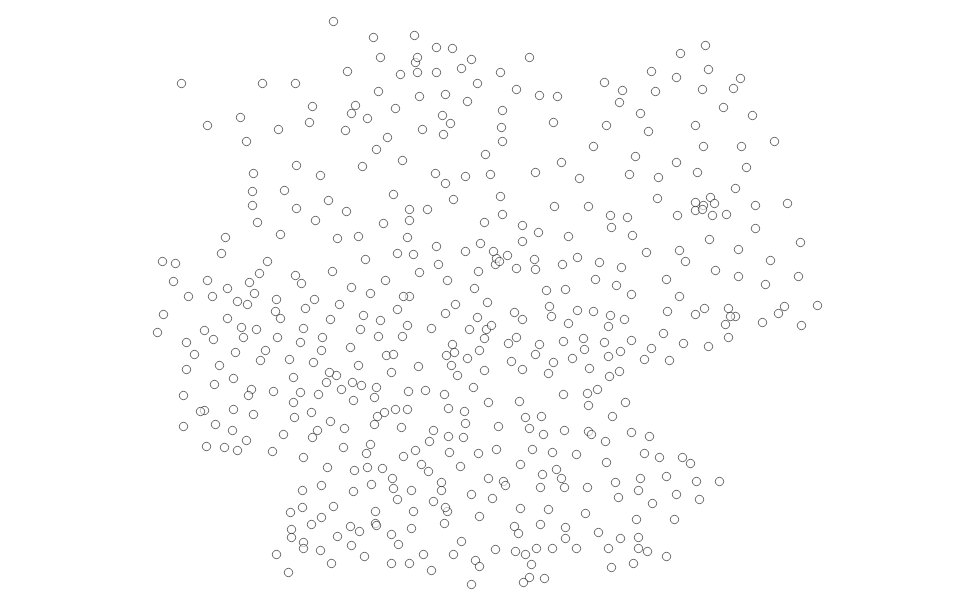
\includegraphics[width=0.8\textwidth]{images/stations.png}
    \caption{weather stations of Deutsche Wetterdienst}
    \label{fig:stations}
  \end{figure}
\end{frame}

\begin{frame}{Data sources - Measurements}
  \headline{Natural Earth \small{Germany}}
  \begin{figure}
    \centering
    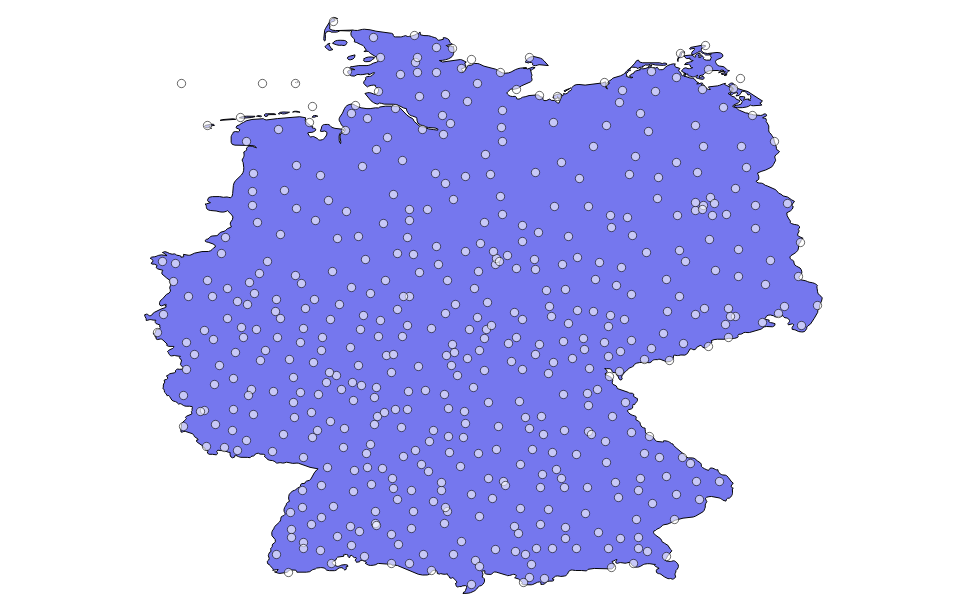
\includegraphics[width=0.8\textwidth]{images/stations_in_germany.png}
    \caption{weather stations on top of polygon of germany}
    \label{fig:germany}
  \end{figure}
\end{frame}

\begin{frame}{Data sources - Measurements}
  \headline{Voronoi}
  \begin{figure}
    \centering
    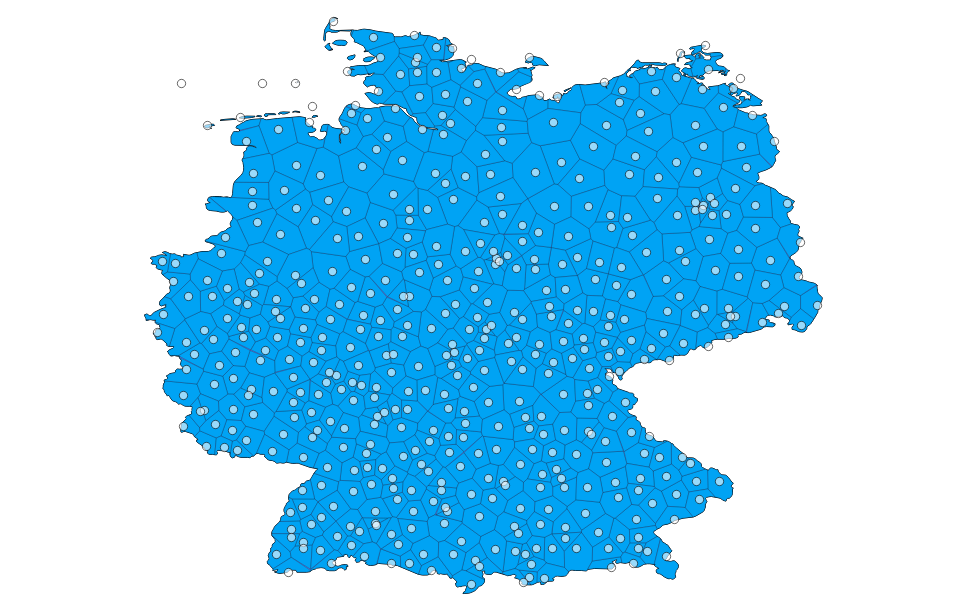
\includegraphics[width=0.8\textwidth]{images/voronoi.png}
    \caption{germany divided into voronoi cells based on weather stations}
    \label{fig:voronoi}
  \end{figure}
\end{frame}

\subsection{Forecast}
\begin{frame}{Data sources - Forecast}
  \begin{block}{NOAA Global forecast system}
    \begin{itemize}
      \item global weather forecast model
      \item data public available for current and past forecasts
      \item data format grib2 (raster)
      \end{itemize}
  \end{block}
\end{frame}

\begin{frame}{Data sources - Forecast}
  \headline{Raster data}
  \begin{figure}
    \centering
    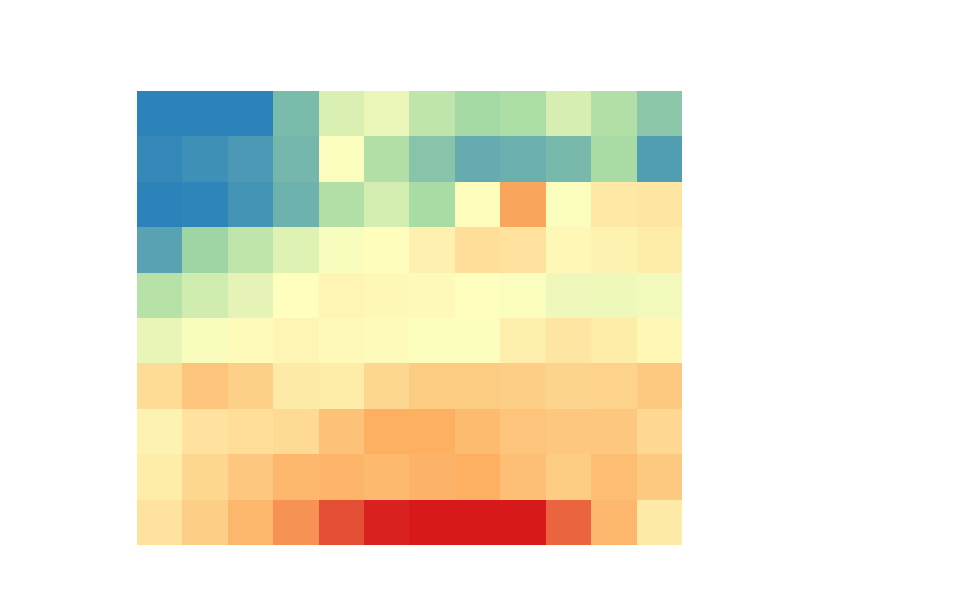
\includegraphics[width=0.8\textwidth]{images/raster.png}
    \caption{24h forecast for \textit{germany} 2015-02-05 18:00}
    \label{fig:voronoi}
  \end{figure}
\end{frame}

\begin{frame}{Data sources - Forecast}
  \headline{Raster data}
  \begin{figure}
    \centering
    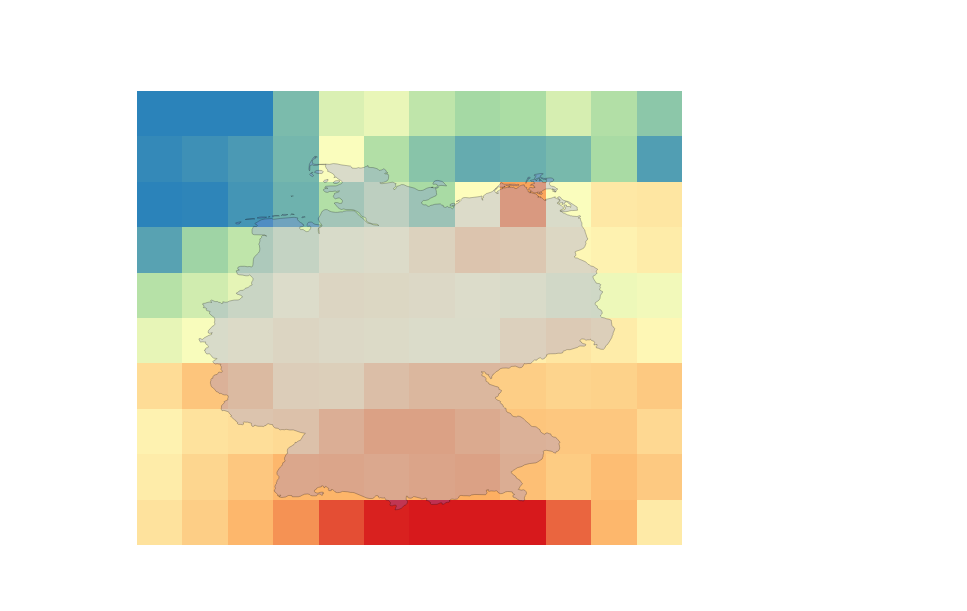
\includegraphics[width=0.8\textwidth]{images/raster_in_germany.png}
    \caption{24h forecast for \textit{germany} 2015-02-05 18:00}
    \label{fig:voronoi}
  \end{figure}
\end{frame}

\begin{frame}{Data sources - Forecast}
  \headline{Raster data \small{resized and resampled (cubic interpolation)}}
  \begin{figure}
    \centering
    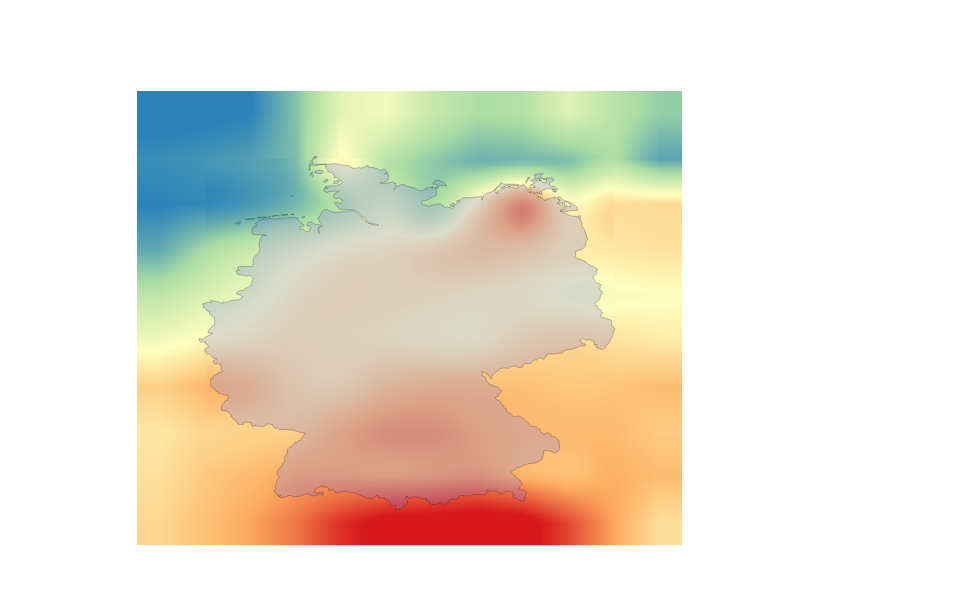
\includegraphics[width=0.8\textwidth]{images/raster_in_germany_resampled.png}
    \caption{24h forecast for \textit{germany} 2015-02-05 18:00}
    \label{fig:voronoi}
  \end{figure}
\end{frame}

\section{Implementation}
\subsection{Schema}
\begin{frame}{Implementation - Schema}
  \begin{block}{Measurement}
    \begin{itemize}
      \item station models weather station
      \item a station measures arbitrary data (measurements)
    \end{itemize}
  \end{block}

  \begin{figure}
    \centering
    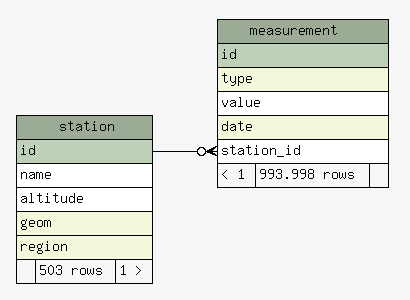
\includegraphics[width=0.4\textwidth]{images/schema_station_measurement.png}
  \end{figure}
\end{frame}

\begin{frame}{Implementation - Schema}
  \begin{block}{Forecast}
    \begin{description}
      \item [date] computation date
      \item [interval] time interval in future
      \item [rast] forecast data in raster format (on several bands)
    \end{description}
  \end{block}

  \begin{figure}
    \centering
    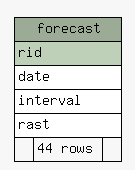
\includegraphics[width=0.2\textwidth]{images/schema_forecast.png}
  \end{figure}
\end{frame}

\subsection{Server}
\begin{frame}{Implementation - Server}
  \begin{block}{Overview}
    \begin{description}
      \item [language] python
      \item [database] postgres+postgis
      \item [architecture] REST api
    \end{description}
  \end{block}

  \begin{block}{Libraries}
    \begin{itemize}
      \item flask web framework
      \item geoalchemy
      \item numpy
      \item shapely
    \end{itemize}
  \end{block}
\end{frame}

\subsection{Client}
\begin{frame}{Implementation - Client}
  \begin{block}{Overview}
    \begin{description}
      \item [language] javascript
      \item [visualization] html/svg
    \end{description}
  \end{block}

  \begin{block}{Libraries}
    \begin{itemize}
      \item leaflet
      \item jquery
      \item spin
    \end{itemize}
  \end{block}
\end{frame}

\section{Presentation}
\begin{frame}{Presentation}
  \center{\Huge{Demo}}
\end{frame}

\begin{frame}{Presentation - Measurements}
  \begin{figure}
    \centering
    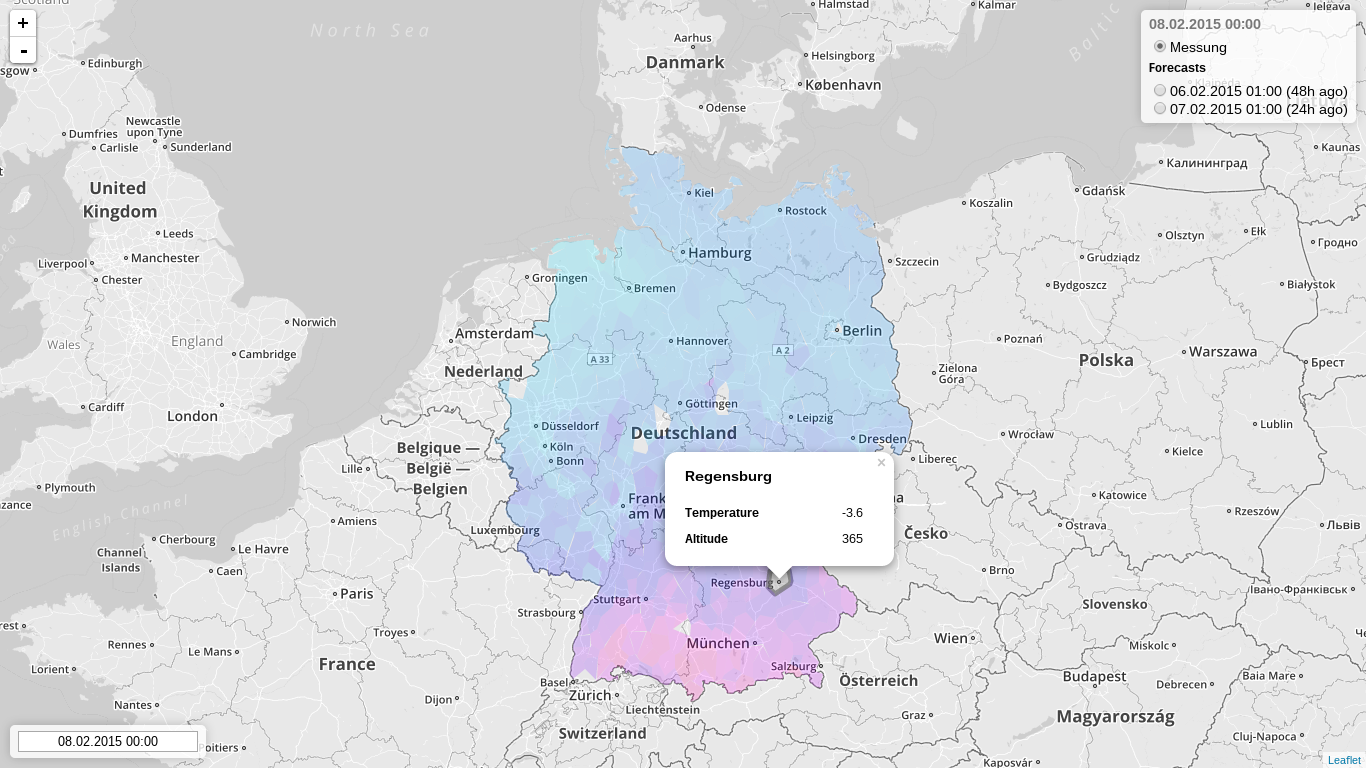
\includegraphics[width=0.8\textwidth]{images/live_measurement.png}
    \caption{weather for germany 2012-02-08 00:00}
    \label{fig:voronoi}
  \end{figure}
\end{frame}

\begin{frame}{Presentation - Forecast}
  \begin{figure}
    \centering
    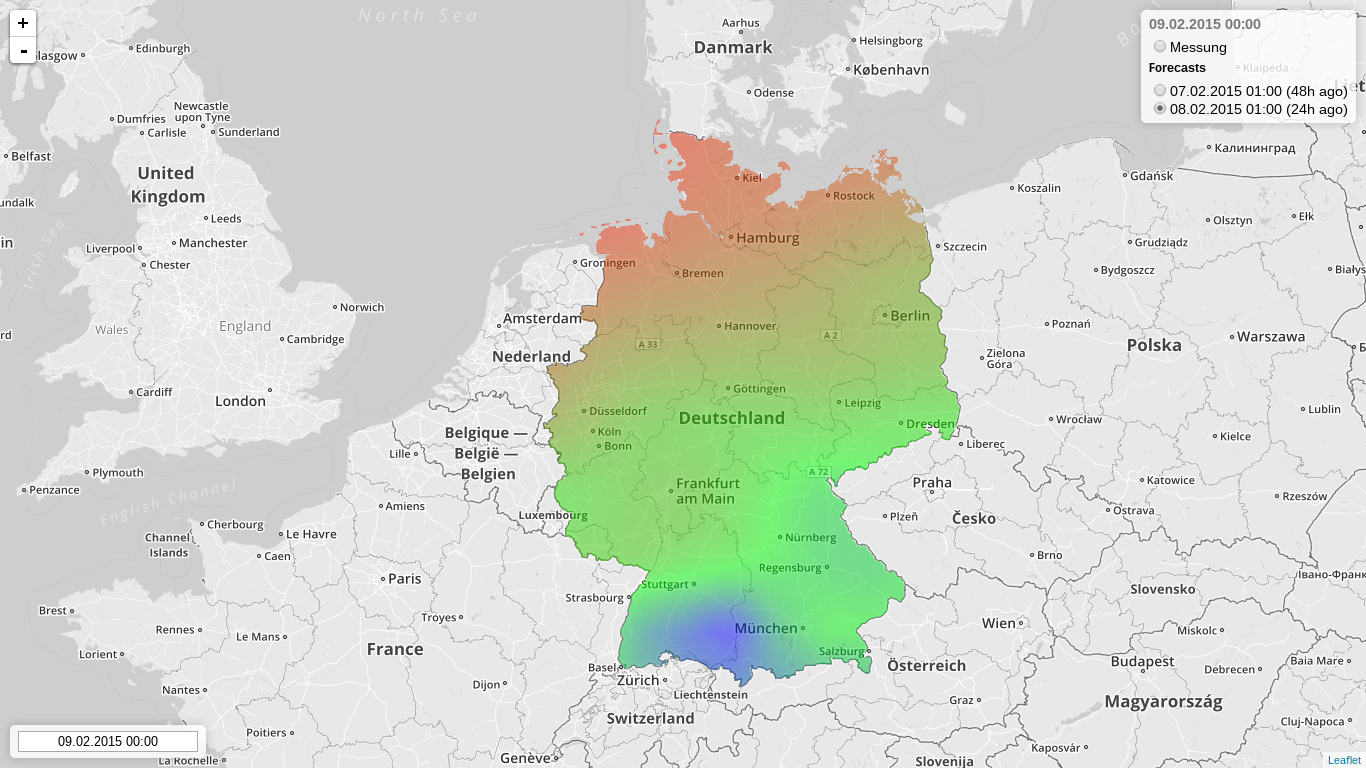
\includegraphics[width=0.8\textwidth]{images/live_forecast.png}
    \caption{forecast for 2015-02-09 00:00 for germany 24h before}
    \label{fig:voronoi}
  \end{figure}
\end{frame}

\section{Outlook and summary}
\begin{frame}{Outlook}
		\begin{block}{Possible extensions}
			\begin{description}
				\item [calculations] creation of own forecast system
				\item [datasets] include and integrate more forecast sources
				\item [visualisation] further features of a weather client
			\end{description}
		\end{block}
\end{frame}

\begin{frame}{Summary}
	\begin{block}{lessons from a mini project}
			\begin{itemize}
				\item learned to account for vector and raster data in postgis
				\item learned latest visualisations frameworks in python
			\end{itemize}
	\end{block}
\end{frame}

\begin{frame}{End}
  \center{\Huge{Question?}}\\
  \center{\huge{Feedback?}}\\
\end{frame}

\end{document}
